\documentclass{school-22.211-notes}
\date{February 22, 2012}

\begin{document}
\maketitle

\topic{Skeleton Spectra Resonance Code}
See slides in Lec 4.
\begin{figure}
  \centering
  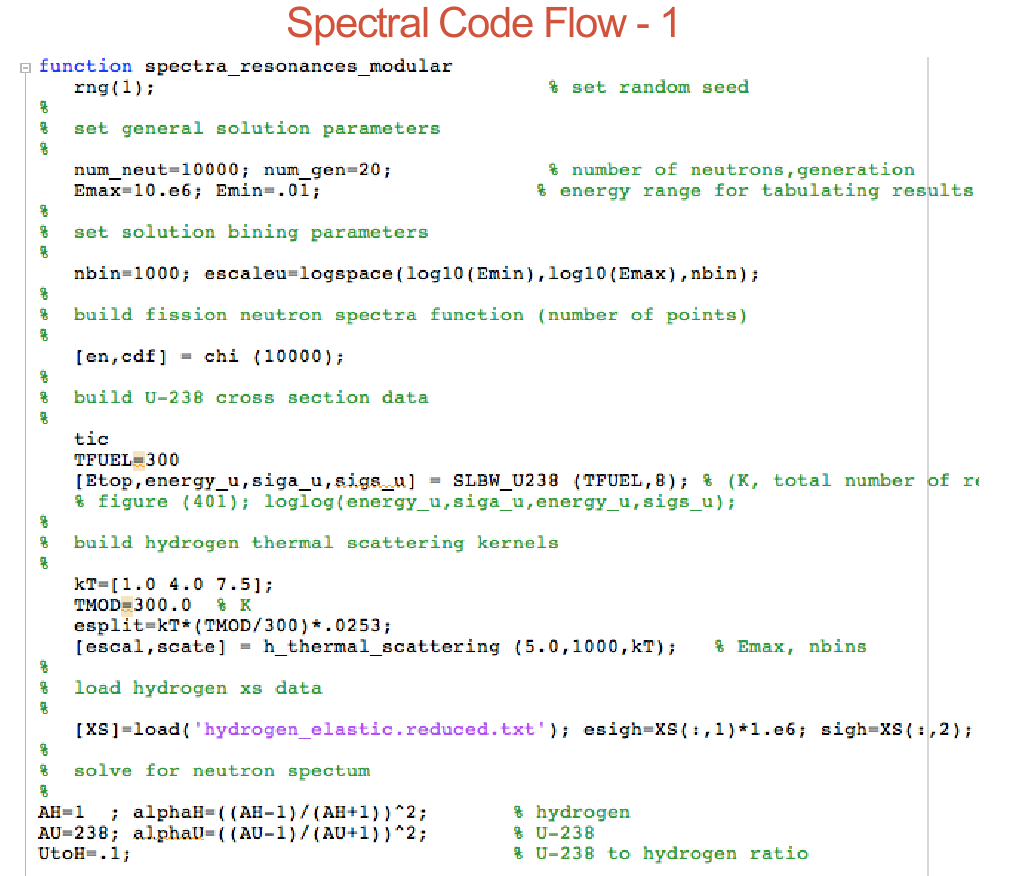
\includegraphics[width=4in]{images/spectral-code-1.png}
  \\
  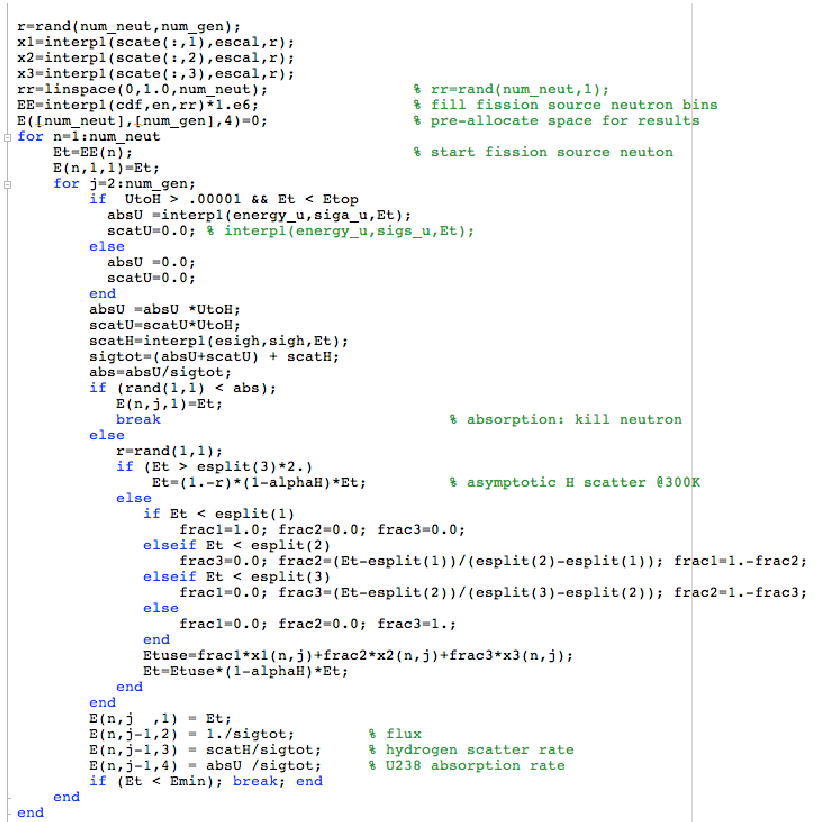
\includegraphics[width=4in]{images/spectral-code-2.png}
  \\
  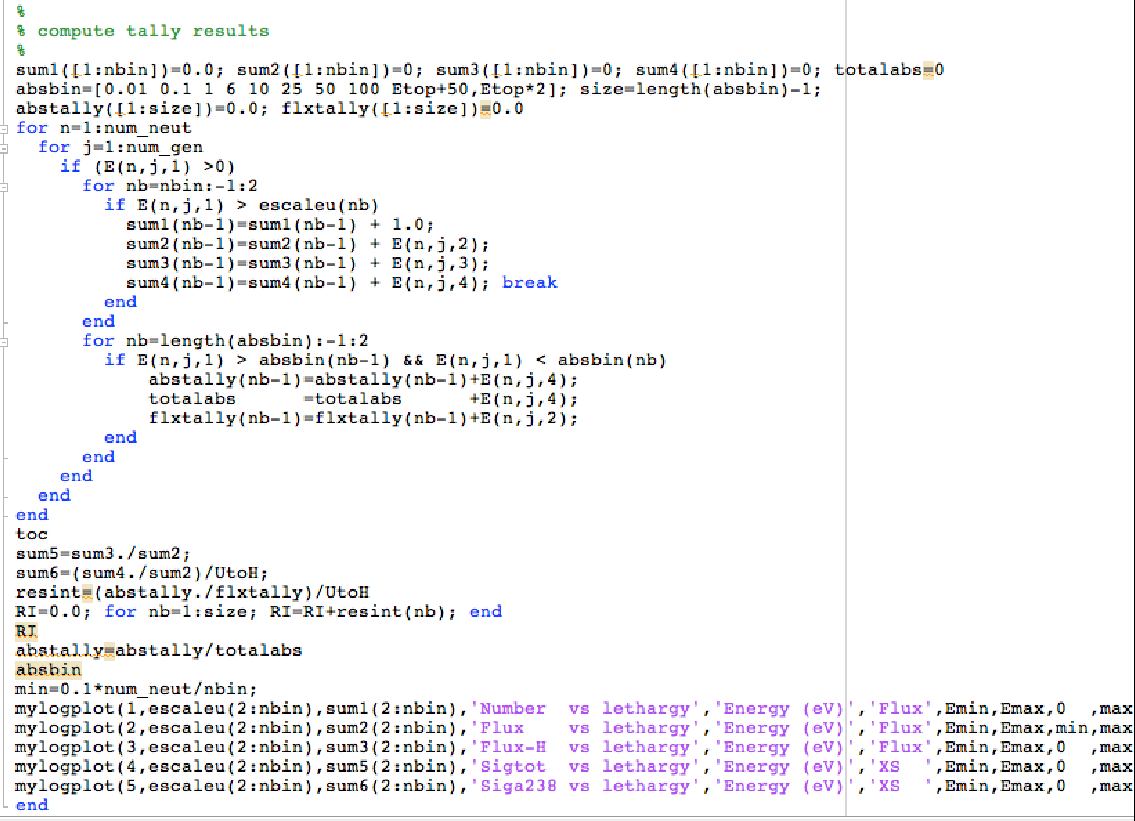
\includegraphics[width=4in]{images/spectral-code-3.png}
  \caption{Skeleton Spectral Code With Resonance}
\end{figure}

\topic{(Infinite) Resonance Integrals vs. Group Cross Section}
We introduce \hi{(Infinite) Resonance Integrals} as flux weighted (that is, weighted with 1/E spectrum $\phi(E) \sim \frac{1}{E}$) microscopic cross section: 
\begin{align}
\RI &=  - \int_{u1}^{u2} \sigma(u) \du \\
u &= \ln \left( \frac{E_0}{E} \right) = \ln(E_0) - \ln E \\
\du &= - \frac{1}{E} \dE \\ 
\RI &=  \int \sigma (E) \frac{1}{E} \dE 
\end{align}
Notice, 
\begin{itemize}
\item RI is defined directly from cross section data; no flux calculation is required because 1/E spectrum is assumed; 
\item RI depends on the normalization of the 1/E flux spectrum; it is also implicitly assumed that flux equals 1 when $E = 1$ through normalization;
\item RI is independent of energy bounds for isolated resonances;
\item RI is independent of temperature. This is because if the energy bound is larger enough, then as temperature increases, the spectrum would broaden, but because the area under the curve remains the same, assume the cross section is constant, then RI is essentially integrating the spectrum, which would not change upon temperature change;
\item RI is useful for inter-comparing libraries or cross section models. It is a classic way to evaluate new resonance data typically from 0.5 eV to 10 keV. We use RI to check our resonance data, in particularly the three big resonances at 6.67, 21, 26 eV. Numerical test of the SLBW RIs shows that the RI comes out to be within 1\% of ENDF/B-VII Reich-Moore data (Lec 6, slide 17, with 0.01 eV as spacing in histogram). 
\end{itemize}

\hi{Group cross section} is a similar but much more useful quantity. From its definition, we see $\sigma_g$ does not depend on the flux normalization: 
\begin{align}
\sigma_g &= \frac{\int_{E_1}^{E_2} \sigma(E) \phi(E) \dE }{\int_{E_1}^{E_2} \phi(E) \dE} 
\end{align}
If we make assumptions on the flux spectrum, then we can relate $\sigma_g$ to $\RI_{\eff}$,
\begin{align}
\phi(E) &\sim \frac{1}{E} \\
\sigma_g &= \frac{\int_{E_1}^{E_2} \sigma(E) \frac{1}{E} \dE }{\int_{E_1}^{E_2} \frac{1}{E} \dE} 
= \frac{\RI_{\eff}}{\ln(E_2) - \ln(E_1)}  
= \frac{\RI_{\eff}}{\ln(E_2/E_1)} \\
\Aboxed{\RI_{\eff} &= \sigma_g \ln(E_2/E_1) } \label{RIeff}
\end{align}
Notice\footnote{Review here for exam}:
\begin{itemize}
\item Group cross section by definition depends on both cross section and flux spectrum. 
\item Group cross section depends on the flux, but not on the normalization of flux (that is, only the shape matters, not the magnitude);
\item Group cross section depend explicitly on energy bounds (widths) of the groups; 
\item Effective RI can be computed from group cross sections and group energy bounds as in Eq.~\ref{RIeff}; As spectrum approaches 1/E, the effective RI computed from group cross sections will approach infinite RI. 
\end{itemize}

\end{document}
